\documentclass[11pt]{article}
\usepackage{basecommon}
\usepackage[margin=1.5in, top=1in]{geometry}
\usepackage[backend=bibtex, natbib=true, autocite=superscript, style=authoryear-ibid]{biblatex}
\usepackage{hyperref}
\usepackage{url}
\usepackage{lineno}
\usepackage{graphicx}
\usepackage{tikz}
\renewcommand{\familydefault}{ptm} % try phv, ptm, ppl
\usetikzlibrary{positioning}
\usetikzlibrary{matrix}
\tikzset{
  treenode/.style = {shape=rectangle, rounded corners,
                     draw, align=center,
                     top color=white, bottom color=blue!20},
  root/.style     = {treenode, font=\Large, bottom color=red!30},
  env/.style      = {treenode},
  result/.style	={treenode, font=\Large, top color=blue!20, bottom color=blue!20}
}
\addbibresource{../ch1/citations_annotated.bib}
\usepackage{setspace}
\doublespacing
\linenumbers
\title{Chapters 3 + 4 (DRAFT - 3/1/16)}
\author{Hugh Zabriskie}
\date{16 February 2015}
\begin{document}
\maketitle{}


\section{Introducing Neural Networks}

I will now shift focus to supervised learning of the chorales using both non-recurrent and recurrent neural models, seeking to improve upon the baseline models presented in Chapter 2. Neural networks are able to engage in sophisticated decision-making by passing the input forward through the network and making more complex and abstract decisions in the hidden perceptron layers. As demonstrated in the literature review at the beginning of Chapter 2, neural networks are popular in computational musicology for their ability to perform highly complex pattern recognition over large datasets and generalize when given unexpected input patterns. In particular, recurrent neural networks (RNNs) show great promise in sequence labelling because of their ability to incorporate contextual information about previous computations. In the case of musical harmony and the task of next-step harmonic prediction, it is critical to understand the local harmonic progression in order to sense the direction of the music. All chords except the tonic generate a sense of tension that insist upon a goal of resolving to the tonic. Therefore, I hypothesize that is critical for the model to understand the tension generated by previous output harmonies when predicting the next harmony. This hypothesis will be evaluated by use of an "Oracle experiment."

\section{Non-Recurrent Models}

The "vanilla" neural network chosen as the non-recurrent model was implemented in Lua using torch7 library. The network has 3 layers, with one layer of varying sizes that was adjusted on the basis of evaluation on a validation set. The validation set consisted of 33 chorales randomly extracted from the training set. A lookup table was added as a layer of convolution that takes the input as a vector of indexed features and outputs a matrix where each column represents an embedding for a feature in the original input. After passing through the hidden layer, the intermediate output is transformed by a softmax to output a probability distribution over all possible output classes. The criterion used was negative log likelihood (NLL), and an NLL value closer to 0 indicates how strongly the model the correct class as its prediction. The objective is to minimize negative log likelihood during training.\\

For each subtask, this model was trained on the same input data $\boldX$ and output data $\boldY$ used in Chapter 2 after GCT was introduced to replace Roman numeral classification. The number of output class for each subtask were 12, 130, 4, 12, and 12, respectively. These models all trained in under a minute, requiring no more than 10 epochs to reach convergence. NLL was reported as an average of over all inputs in the training and test sets.

 \begin{table}[h]
\begin{center}
\caption[Table caption text]{\textbf{"Vanilla" neural network accuracy.}}
\begin{tabular}{l *{4}{c}}
Task & Training NLL & Acc\% & Test NLL & Acc\% \\ \hline
Root & 0.865 & 68.92\% & 1.106 & 60.86\% \\
Base & 1.402 & 62.10\% & 1.686 & 57.83\% \\
Inversion & 0.675 & 73.26\% & 0.785 & 69.67\% \\
Alto & 1.473 & 59.22\% & 1.710 & 56.27\% \\
Tenor & 1.320 & 52.91\% & 1.751 & 40.05\% \\
\end{tabular}
\end{center}
\end{table}

\textbf{Update these values. They might have been from the Oracle experiment and were mislabeled.}

\subsection{Full Harmonization}

The baseline models and the neural network were also trained on the "full harmonization task", where the output represented a full set of decisions for all subtasks. Each full set of decisions in the training set is assigned a unique class index. For the test set, only inputs that map to an index in the training set are used. To understand why, imagine a model that took an image as input and predicted whether the image depicted a cat, dog, or bird. If during training the model, only images of cats and dogs are shown, then the model will gradually adjust its weights to reflect the fact that bird is never right answer. Therefore, if the model is tested on an image of a bird, it is extremely improbable that the model will guess correctly because of the data it was trained on. Similarly, the neural network will not guess the correct full harmonization class if it never appeared during training. \\

The network was trained until convergence around 20 epochs, and the code is in the script \texttt{eval-sm.lua}. Random forests and neural networks continue to outperform the other models, although Random forests consistently achieving a slightly higher accuracy. The results for multinomial naive Bayes, the worst performer on average, were therefore left out. \\

 \begin{table}[h]
\begin{center}
\caption[Table caption text]{\textbf{"Vanilla" neural network accuracy, full harmonization task.}}
\begin{tabular}{l *{4}{c}}
Classifier & Test NLL & Acc\% \\ \hline
Multiclass Logistic & -- & 6.26\% \\
Random Forest & -- & 31.35\% \\
Neural Network & 4.614 & 26.35\% \\
\end{tabular}
\end{center}
\end{table}

There are two significant flaws to this approach. First, the accuracy metric here is harsh because by combining a series of decisions into a single class, a much more fine-grained decision must be made to choose the correct class. This could be improved by creating a more sophisticated accuracy metric that took into account its overall accuracy across all subtasks. Second, I hypothesized that the model would be improved significantly if after the model output a decision for a subtask that that information would be provided as part of the input for the next subtask. This hypothesis reflects the musician's method of harmonization, where, for example, knowing that the next chord should be in terms of its root and base will significantly influence the selection of the alto and tenor pitches. \\

A new approach was therefore taken for deciding a full harmonization at each time step. Figure 1 shows the sequence of decisions that comprises the complete harmonic decision for a given time step. This decision process acknowledges the \textit{dependent} nature of the subtasks, and therefore the ordering of their completion influences the model performance. This ordering decides the harmony in the two subtasks, while the final three decide the specific notes to voice that harmony. The final two are hypothesized to be interchangeable, since the Alto and Tenor voices are traditionally inner voices are relatively equal weight.

Let's assume for the sake of shorthand that there are only three subtasks. Then the objective is to select
$$\argmax_{x, y, z} P(X=x, Y=y, Z=z | \boldX)$$ 

where X, Y, and Z are each random variables associated with a specific subtask and can only have the value of a class belonging to the variable's subtask, and $\boldX$ represents the initial input data. Let $\hat{x}, \hat{y}, \hat{z}$ be the predicted classes for the 3 subtasks. By the chain rule, we can show that Then by the chain rule,
\begin{align*}
\hat{x}, \hat{y}, \hat{z} &= \argmax_{x, y, z} P(X=x, Y=y, Z=z | \boldX) \\
				  &= \argmax_{x,y,z} P(X=x | \boldX, Y=y, Z=z) \cdot P(Y=y | \boldX, Z=z) \cdot P(Z=z | \boldX)
\end{align*}

More work needs to be done to evaluate this model and ensure it is working probably. During training, the each subtask is fed the original input data along with the correct classes for the previous subtasks in the sequence. During test time, its decision for each subtask is propagated through future decisions. The possible choices of $x,y,z$ are selected from the combinations of outputs seen in the training set. But as of now, this model achieves around 40\% accuracy across subtasks.

\begin{figure}[h]
\begin{center}
\caption{\textbf{Sequence of harmonization subtasks with dependent decision making.}}
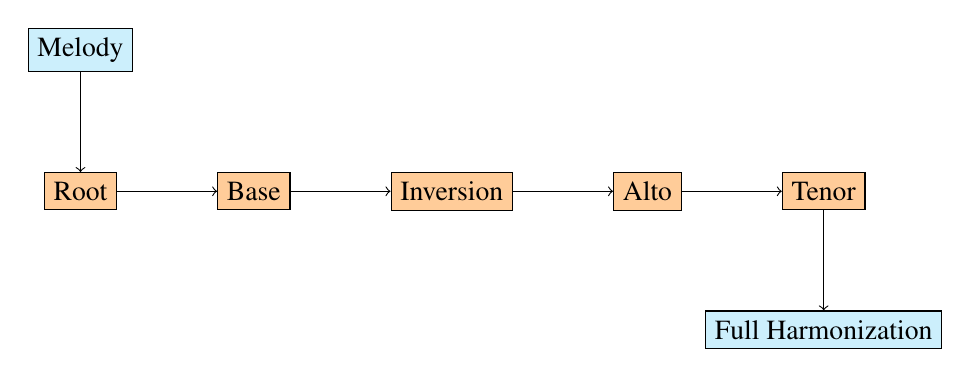
\begin{tikzpicture}
  [
    grow                    = down,
    sibling distance        = 6em,
    level distance          = 4em,
    edge from parent/.style = {latex-latexnew, line width=2pt, arrowhead=4cm}
  ]
  \begin{scope}[end/.style={rectangle,draw,fill=cyan!20},
  			env/.style={rectangle,draw,fill=orange!40}, node distance=1in]
  \node [end] (mel) {Melody};
  \node [env] (a) [below=0.5in of mel] {Root};
  \node [env] (b) [right=0.5in of a] {Base};
  \node [env] (c) [right=0.5in of b]{Inversion};
  \node [env] (d) [right=0.5in of c] {Alto};
  \node [env] (e) [right=0.5in of d] {Tenor};
  \node [end] (f) [below=0.5in of e] {Full Harmonization};
  \path[->] (mel) edge node {} (a);
  \path[->] (a) edge node {} (b);
  \path[->] (b) edge node {} (c);
  \path[->] (c) edge node {} (d);
  \path[->] (d) edge node {} (e);
  \path[->] (e) edge node {} (f);
  \end{scope}
\end{tikzpicture}
\end{center}
\end{figure}

\section{Recurrent Models}

\subsection{Oracle experiment}

Before, applying RNNs to this task, I wanted to know if having the context of previous harmonies would in fact improve the model. An Oracle experiment is so-called termed in the field of natural language processing because there is the addition of an "oracle" in the data that always provides the correct answer. It is used to compare one system to another system by including the "oracle" and evaluating how your model responds when one component of it always provides the correct answer. Such an experiment is performed here to determine whether the neural model presented in the previous section will perform better with this knowledge. If so, it would strongly suggest that the context provided by a recurrent model would improve results.

In \texttt{featurize.py}, the final three columns of $\boldX$ describe the correct harmony (root, base, and inversion) at time step $t-1$. This information simulates the additional information provided in a recurrent model from the computation at the previous time step. The baseline models were re-evaluated on this dataset as well as the neural model, using the same training-test split as a GCT-updated dataset described in Chapter 2.

\begin{table}[h]
\begin{center}
\caption[Table caption text]{\textbf{Baseline and neural model test accuracy, Oracle experiment}}
\begin{tabular}{l *{5}{c}}
Classifier & Root & Base & Inversion & Alto & Tenor \\ \hline
Multi-Class Logistic & 59.75\% & 56.49\% & 64.43\% & 43.36\% & 38.93\% \\
Multinomial Naive Bayes & 52.62\% & 50.08\% & 63.05\% & 38.58\% & 35.93\% \\
Random Forests & 68.85\% & 61.37\% & 68.45\% & 51.96\% & 49.01\% \\ \hline
Neural Network & 60.86\% & 57.83\% & 69.67\% & 56.27\% & 40.05\% \\
\end{tabular}
\end{center}
\end{table}

\textbf{TODO: re-run neural network values for Oracle experiment}


\subsection{RNN Implementation}

Based on the promising results of the Oracle experiment, I constructed a recurrent neural network in Torch to determine if RNNs would improve accuracy over a \textit{sequence} of inputs. As discussed in Chapter 1, RNNs include recurrent connections that allow for feedback from the computation that occured at the previous time step. During the forward pass, at each time step in the data sequence, the RNN input layer receives an external input from the $i$th sequence $x^{(i)}_t$ as well as internal feedback from the hidden layer $h_{t}$, and then outputs a distribution $x_{t+1}$ for the next time step. Here, each element of the sequence is a feature vector describing a single melody note, drawn from the same dataset used for previous models.
\begin{center}
\begin{tikzpicture}
  \matrix (m) [matrix of math nodes,row sep=3em,column sep=4em,minimum width=2em]
  {
     time \to & h_t & \to\\ 
     x^{(i)}_t & RNN & x^{(i)}_{t+1}\\
     \to & h_{t+1} & \to\\};
  \path[-stealth]
    (m-1-2) edge (m-2-2)
    (m-2-1.east|-m-2-2) edge [double] (m-2-2)
    (m-2-2.east|-m-2-3) edge [double] (m-2-3)
    (m-2-2) edge (m-3-2);
\end{tikzpicture}
\end{center}

Each chorale represents an independent sequence that is fed into RNN and outputs a synced sequence of distributions that correspond to the probability of each possibility harmonization at each time step. The most likely harmonization for each time step is chosen by taking the $\argmax$ of that time step's output distribution, $x^{(i)}_{t+1}$.

$$\argmax x^{(i)}_{t + 1} = \argmax_k
\begin{bmatrix} x^{(i)}_{{t+1}_1} \\ x^{(i)}_{{t+1}_2} \\ \vdots \\ x^{(i)}_{{t+1}_k}
 \end{bmatrix}
 $$

Internally, $h_t$ is a stored as a "memory" of the melody features at time $t + 1$, which will be used to predict the harmonization $x_{t+2}$. \\

As a preprocessing step, each chorale was "padded" to the length of the longest chorale (in this dataset, this was 208 segments). The padding was added to all chorale sequences (both input and output vectors) using a unique "padding" feature in order not to confusing the padding with the actual musical section of the sequence. The output sequence was the same as the full harmonization task described in section 2.1 of Chapter 3, where each feature denotes a full set of harmonic decisions, including the notes for the harmonizing notes as well as a complete harmonic labelling using the GCT notation. Table 4 contains the results.

\begin{table}[h]
\begin{center}
\caption[Table caption text]{\textbf{Neural and baseline model accuracy, full harmonization task}}
\begin{tabular}{l c c c }
Model & Train NLL & Train & Test \\ \hline
Multinomial Logistic & -- & 42.74\% & 25.15\% \\
Random Forests & -- & 89.83\% & 33.41\% \\ \hline
LSTM & 0.807 & 38.01\% & 29.35\%
\end{tabular}
\end{center}
\end{table}

Given that the MFFC frequency is 5\%, these results show a significant increase in accuracy over previous results. The random forest model continues to outperform neural models based on accuracy, potentially for reasons related to imbalanced data, as discussed in Chapter 2. 

\newpage

\section{Chapter 4 - Looking forward}

\subsection{Further Exploration: The Bach Inventions}

It must be admitted that a model trained to harmonize chorales has limited utility in modern times (although it might have made Bach's work as \textit{Kapellmeister} a bit easier). Musicians only look to Bach's chorales as early model compositions for 4 voices and for theory-related exercises. Moreover, the Chorales themselves use a limited rhythmic and textural vocabulary, since they remain harmonically close to the tonic key and the rate of harmonic change is consistent, and highly variable in almost all other repertoire. <-- \textbf{FIX THIS LINE} This simplicity makes the chorales advantageous for statistical learning and allows our models to output a uniform set of harmonizations over all inputs. But as chorale harmonization is increasingly well-understood as a computational task, it is worth recognizing the ways in which these models can be extended to more common musical processes. As one potential application of these models, I will explore the task of composing a counterpoint line given an input melody, and how this might be approached from a computational standpoint. This task is intentionally general and could be applied to a wide variety of well-known musical corpora. But here, I will focus on Bach's 15 Inventions because they are a body of exemplary two-voice counterpoint compositions by the same composer who wrote the Chorales. Despite being written explicitly as musical exercises, they are far more melodically and rhythmically complex than the Chorales.

\subsubsection{Added complexity}
Generating harmonizations for inventions introduces several new layers of musical complexity that were not considered when harmonizing the chorales. One is rhythmic complexity, since Invention melodies cannot be easily abstracted into units of a single rhythmic length. One method for describing rhythm in the generated melody is by generating predictions at the level of the smallest rhythmic unit. For example, if the smallest rhythmic unit in the composition is the 32nd notes, then each measure would be divided into 32 samples. Then after a prediction, \textbf{FINISH THIS SENTENCE} determining the duration of the pitch based on the number of iterations that the same pitch is consecutively output by the model. \citet{eck2002blues} found this approach effective for composing blues melodies. An similar but alternative model was proposed by \citet{franklin2006jazz}, where separate LSTMs are trained to decide pitch and duration. An additional layer complexity is the large-scale structure of the Invention. Inventions typically consist of a series of thematic statements interleaved with episodes - modulatory sections that are melodically derived from the subject and create transitions between thematic statements in different keys. The remaining sections might be termed "elaborations", which include cadences at the ends of episodes and codettas that occasionally come at the end of an Invention. Each type of section has a specific set of conventions that govern its structure as well as the relationship between the two voices. A final layer of complexity to note is the need for subject identification. In contrast to the Chorales, a single melodic idea (the "invention", or subject) governs the development of the entire work, and it is consistently restated in various transformations (\textbf{check about "invention" in Dreyfus, does it mean a subject or more like elaboration? find a quote}). Identification of the subject is essential for determining the melodic, harmonic, and rhythmic material used in the Invention, and features from the subject should be extracted to create contrapuntal melodies.

\subsubsection{Subject identification}
Bach's Inventions are two-voice compositions, where the lower voice can be characterized as a \textit{function} of the upper voice. In order for the model to learn the harmonic and rhythmic material that Bach employs in the work, the model should first identify and extract features from the Invention's primary \textit{subject}. Identifying the subject generally straightforward for the listener, since the primary subject is typically the first statement in the upper voice. However, inventions can contain multiple subjects with varying levels of importance. And in Invention No. 6 in E major, Bach introduces two subjects of equal importance and develops them both consistently throughout. Therefore, a better approach might be to identify subjects by selecting melodic ideas based on the frequency with which they are restated. \citet{dreyfus1996bach} notes that the frequency of a subject is directly correlated with its importance in the Invention - a principle of repetition that is generally true of melodies in Western music. One candidate algorithm for subject identification based on repetition is hierarchal agglomerative clustering (HAC), which can learn to "cluster" melodic segments based on a supplied distance metric. \citet{nagler2014schubot} applied HAC to the task of motivic analysis in Schubert's song cycle \textit{Die Winterreise} and found promising results in extracting the main motive from each song. However, a significant difficulty in subject identification would be the harmonic and rhythmic transformations that are often applied to the subject when it is restated. For this task, it could be useful to encode the melody as a series of intervals rather than pitches in order to identify subjects in their original form as well as their transformed state. \\

\begin{figure*}[h]
\caption{ The subject and transformations in Invention No. 4 in D Minor, BWV 775.  }
\centerline{\includegraphics[scale=0.3]{examples/ex1}}
\end{figure*}


\subsubsection{Form identification}
Once rhythmic and melodic features are extracted from the most prominent subjects, the model can use these to analyze the large-scale structure of the Invention and divide the work into a series of sections. One classifier could be trained to create the general boundaries of each section, while a separate classifier could label each section as a thematic statement ($T$), episodes ($S$), and elaborations ($E$) by analyzing if and how the subject is presented in the upper voice. Complete, sequential statements of the subject suggest a thematic statement, while partial and transformed subject statements will suggest an episode. Elaborations will most likely differentiate themselves by the unique and less repetitive melodic material.

\subsubsection{Harmonic identification}
Before generating the melody, a useful preprocessing step would be to perform harmonic analysis over the upper voice. The classifier would be trained to accept the upper voice as input and output a sequence of corresponding harmonic encodings. This task is well-suited to the model presented in Chapter 2 and 3, where information about a segment of the melody would be classified as a GCT-encoded harmony. While many pleasant melodies can be generated for the counterpoint melody, the most crucial constraint is harmonic agreement. A crucial purpose of the contrapuntal lower voice is to support the upper voice in harmony. The upper voice typically guides the progression, while the lower voice may echo and reinforce harmonic transitions, as Figure 3a illustrates. \\

The primary technique for implying harmonies is the use of scalar and triadic passages. Not coincidentally, many of Bach's subjects are constructed to facilitate various transformations (\textit{SHIFT}, \textit{INV}, \textit{AUGMENT}, etc.) and be harmonically indicative. However, given a scalar or triadic passage, it can be difficult to determine which of many potential chords is most strongly implied. There are several important indicators, including the harmony in the previous melodic unit and the beat strength of the notes in the current unit. A recurrent model would likely perform well on this task because of the sequential format of the data (representing the upper voice as a \textit{sequence} of melodic units) and the feedback loop that would provide information about preceding harmonies. The size of each melodic unit, however, is an additional parameter that would require adjustment since the implied harmonies have varying durations (Figure 3b). \\

\begin{figure*}[h]
\caption{ Excerpts from Invention No. 13 in A Minor, BWV 784.  }
\centerline{\includegraphics[scale=0.27]{examples/ex2}}
\end{figure*}

\subsubsection{Contrapuntal melodic generation}
Using the structural information gathered during preprocessing, a final classifier is trained to generate contrapuntal melodies. The classifier would accept input features describing the current relevant subject, the current section of the form, and the current implied harmony, as well as melodic features related to the upper voice near time $t$. The output feature would describe the most likely pitch for time $t$, with an implied duration of the length of the time step. Consecutive time steps of the same pitch could be merged to represented longer notes. \\
The generalization of this model allows for a wide range of corpora to be incorporated into the training data. Stylistically similar candidates include Bach's Sinfonias (the 3-voice equivalent of the Inventions) and the Fugues. Stylistically separate candidates include Palestrina's masses and motets, which feature significant contrapuntal composition and development of melodic motives in multiple voices. The larger dataset available for training will very likely improve model performance, in comparison to the computationally small dataset of chorales used in this paper. Further work should be done to explore this extension of the harmonization task to various musical corpora.

\newpage

\subsection{Conclusion}

In this paper, the objective was to apply a variety of neural and non-neural models to different musical processes involved in the task of chorale harmonization. These models are meant to supplement existing work on computational approaches to generative and completive musical tasks, not to replace human musical analysis or composition. The Random forest model and recurrent neural models proved most effective in learning the various subtasks associated with harmonization, and in the future they should be evaluated on similar musical tasks, such as the generation of contrapuntal voices. The accuracy results from experiments with these computational models demonstrate a promising ability to learn musical structure and connect temporally distant events.

\subsection{Code and related files}

All code and data related to this paper is freely available on GitHub at\\ \url{https://github.com/glasperfan/thesis/}.

\newpage

\printbibliography

\end{document}